% Arbeit.tex
% LaTeX-Hauptdatei fuer Studien/Diplomarbeiten am IMMD 9
% geschrieben von Wolfgang Heidrich <wgheidri@immd9.informatik.uni-erlangen.de>
% erweitert von Christian Vogelgsang <cnvogelg@immd9.informatik.uni-erlangen.de>
% und von Darius Rückert <darius.rueckert@fau.de>

% benoetigt LaTeX 2e (z.B. in teTeX)

% --- Style + Optionen ---
% Font: 11pt bevorzugt, 10pt fuer besonders lange Arbeiten.
%       12pt nur in Ausnahmefaellen.
\documentclass[11pt, twoside, openright, a4paper]{studdipl} 

% --- Paketauswahl ---
% a4wide: breites Papierformat
% german: Deutsche Ueberschriften
% epsfig: figures mit EPS Bilder
\usepackage{a4wide}

%\usepackage{biblatex}
\usepackage[
backend=biber,
style=numeric,
bibencoding=utf8
]{biblatex}
\addbibresource{Literatur.bib}

%%%%%%%%%%%%%%%%%%%%
% nice libraries. Use what you want

\usepackage{graphicx,import}
\usepackage{color}
\usepackage{booktabs}
\usepackage[hidelinks]{hyperref}
\usepackage{todonotes}
\usepackage{siunitx}
\usepackage{amsfonts}	
\usepackage{amsmath}
\usepackage{amssymb}
\usepackage{wrapfig}
\usepackage{multirow}
\usepackage{listings}
\usepackage{algorithmic}
\usepackage[boxed,chapter]{algorithm}
\usepackage{subcaption}
% \caption zb. in \figure wird \small
\usepackage[margin=10pt,font=small,labelfont=bf]{caption}		
\usepackage{pgfplots}
\usepackage{filecontents}
\usepackage{tikz}
\usetikzlibrary{shapes,arrows}
\usetikzlibrary{positioning}
\usetikzlibrary{calc}

% danke, daniel:
\lstdefinelanguage{CUDA}{morekeywords={
	__device__, __global__, __host__, __constant__, __shared__, __noinline__,
	__syncthreads, __any, pragma, unroll, extern,
	gridDim, blockIdx, blockDim, threadIdx, warpSize,
	min, max, abs, sqrt, exp, pi, pow, log, floor,
	char1, uchar1, char2, uchar2, char3, uchar3, char4, uchar4,
	short1, ushort1, short2, ushort2, short3, ushort3, short4, ushort4,
	int1, uint1, int2, uint2, int3, uint3, int4, uint4,
	long1, ulong1, long2, ulong2, long3, ulong3, long4, ulong4,
	float1, float2, float3, float4, double2, dim3,
	texture, tex1Dfetch, tex1D, tex2D, tex3D,
	cudaReadModeElementType,
	atomicAdd, atomicExch,
	CUresult, CUdevice, CUcontext, CUmodule, CUfunction, CUtexref,
	cuInit, cuDeviceGetCount, cuDeviceGet,
	cuCtxCreate, cuCtxPushCurrent, cuCtxPopCurrent, cuCtxAttach, cuCtxDetach, cuCtxDestroy,
	cuModuleLoad, cuModuleGetFunction,
	cuParamSeti, cuParamSetf, cuParamSetv, cuParamSetSize
}}

\lstdefinelanguage{Scheme}{morekeywords={
	define, begin, if, display, newline, let*, or
}}

% settings for listing environment
\lstset{language=C++,
		alsolanguage=CUDA,
		basicstyle=\small,
		frame=single,
        breaklines=true,
        breakatwhitespace=true,
		numbers=left,
		numberstyle=\tiny,
		xleftmargin=5mm,
		captionpos=b,
		tabsize=4
}

%%%%%%%%%%%%%%%%%%%%

% --- CV Config: ---

% --- weitere Pakete ---

% inputenc: direkte Eingabe von Umlauten erlaubt!
\usepackage[utf8]{inputenc}
% huebsche Rahmen fuer Sourcecodebloecke
\usepackage{fancybox}
\usepackage{bm}

% --- Optionen ---

% steuert das Figure Placement auf den Seiten
\renewcommand{\floatpagefraction}{0.8}

% definiert die Kopfzeile
\lhead[]{\fancyplain{}{\rightmark}}
\rhead[{\fancyplain{}{\leftmark}}]{}

% --- CV Config Ende ---

% Ein wenig liberalere spacing rules
\frenchspacing

\DeclareRobustCommand{\uvec}[1]{{%
		\ifcsname uvec#1\endcsname
		\csname uvec#1\endcsname
		\else
		\bm{\hat{\mathbf{#1}}}%
		\fi
}}

% Matrix: Capital Letters + Fat
\newcommand{\myMatrix}[1]{\bm{\mathit{#1}}}
% Vector: Small letters + Fat
\newcommand{\myVector}[1]{\bm{\mathit{#1}}}
% Scalars: Small letters + thin


% Erlaube groessere Freiraeume zwischen Woertern.
% (wichtig fuer Deutsche Texte wegen der grossen durchschnittlichen
% Wortlaenge). Fuer Englische Arbeiten moeglicherweise weglassen.
% \sloppy

\graphicspath{{../images/}}

% -------------- Konfiguration ------------------------------------------------

\thesistype{Master project}

% Titel der Arbeit
\title{Predict lidar in multi weather senaros}

% AutorIn <- Dein Name :-)
\author{Behrooz bozorgchamy}

% Dein Geburtsdatum
\birthday{30-09-1998}

% Dein Geburtsort:
\birthplace{Tehran-Iran}

% DeinE BetreuerIn:
\supervisor{Richard Marcus}

% Beginn der Arbeit
\bdate{April 2024}

% Abgabetermin
\edate{July 2024}

% -------------- Ende der Konfiguration ---------------------------------------

\setcounter{secnumdepth}{3}

\begin{document}


% DRAFT MODE
% Erzeugt eine Ueberschrift mit dem Datum des Drafts. Muss fuer die
% endgueltige Version natuerlich auskommentiert werden!!!
%\draft

% Der "Vorspann" hat roemische Seitennummern 
\prepages

% short mode: uncomment
% Damit wird die zweite Titelseite erstellt (die erste ist ja in einem
% separaten File)
\maketitle

% eine Leerseite
\cleardoublepage

% Inhaltsverzeichnis
\tableofcontents

% eine Leerseite
\cleardoublepage
% end of short mode

% der eigentliche Text hat arabische Nummern
\mainbody

% ---------- Kapitel ---------

\begin{abstract}
	The purpose of this project is improve prediction of cloud point image in per weather condtions. To achieve this, we use a multi weather condtions dataset and change some models to get a weather mask as another input. Our results show that models can prediction better when the camera image has some distorted. These findings suggest that model prediction cannot be better in some weather condtions but it can help to reduce camera distorted. Keywords: Multiweather, boreas, LIdar.
\end{abstract}

\chapter{Introduction}
\label{chap:intro}

\section{Motivation}
\label{sect:motivation}
The performance of Lidar point clouds can be significantly affected by various weather conditions. For instance, in snowy weather, the presence of snowflakes on the surface can cause light reflections in different directions, leading to inaccuracies in the data. Similarly, in sunny weather, the shadows cast by vehicles can mimic the effects seen in rainy conditions, resulting in false predictions by the model. Additionally, camera images can encounter issues due to lens obstructions caused by rain or snow, which can lead to unclear or distorted visuals.

Moreover, foggy conditions can reduce the range and accuracy of Lidar sensors, as the dense particles in the air scatter the laser beams. This scattering effect can cause the Lidar to misinterpret the distance and shape of objects. Windy conditions can also introduce noise into the data, as moving debris or leaves can be mistakenly identified as obstacles.

Furthermore, the accumulation of dirt or water droplets on the Lidar sensor or camera lens can degrade the quality of the data collected. Regular maintenance and cleaning of these sensors are crucial to ensure optimal performance but It is not an easy job in  moving vehicle. Advanced algorithms and machine learning models are being developed to mitigate these weather-related issues, but challenges remain in achieving consistent accuracy across all conditions.
\begin{figure}[!ht]
	\begin{minipage}[t]{.45\linewidth}
		
		
		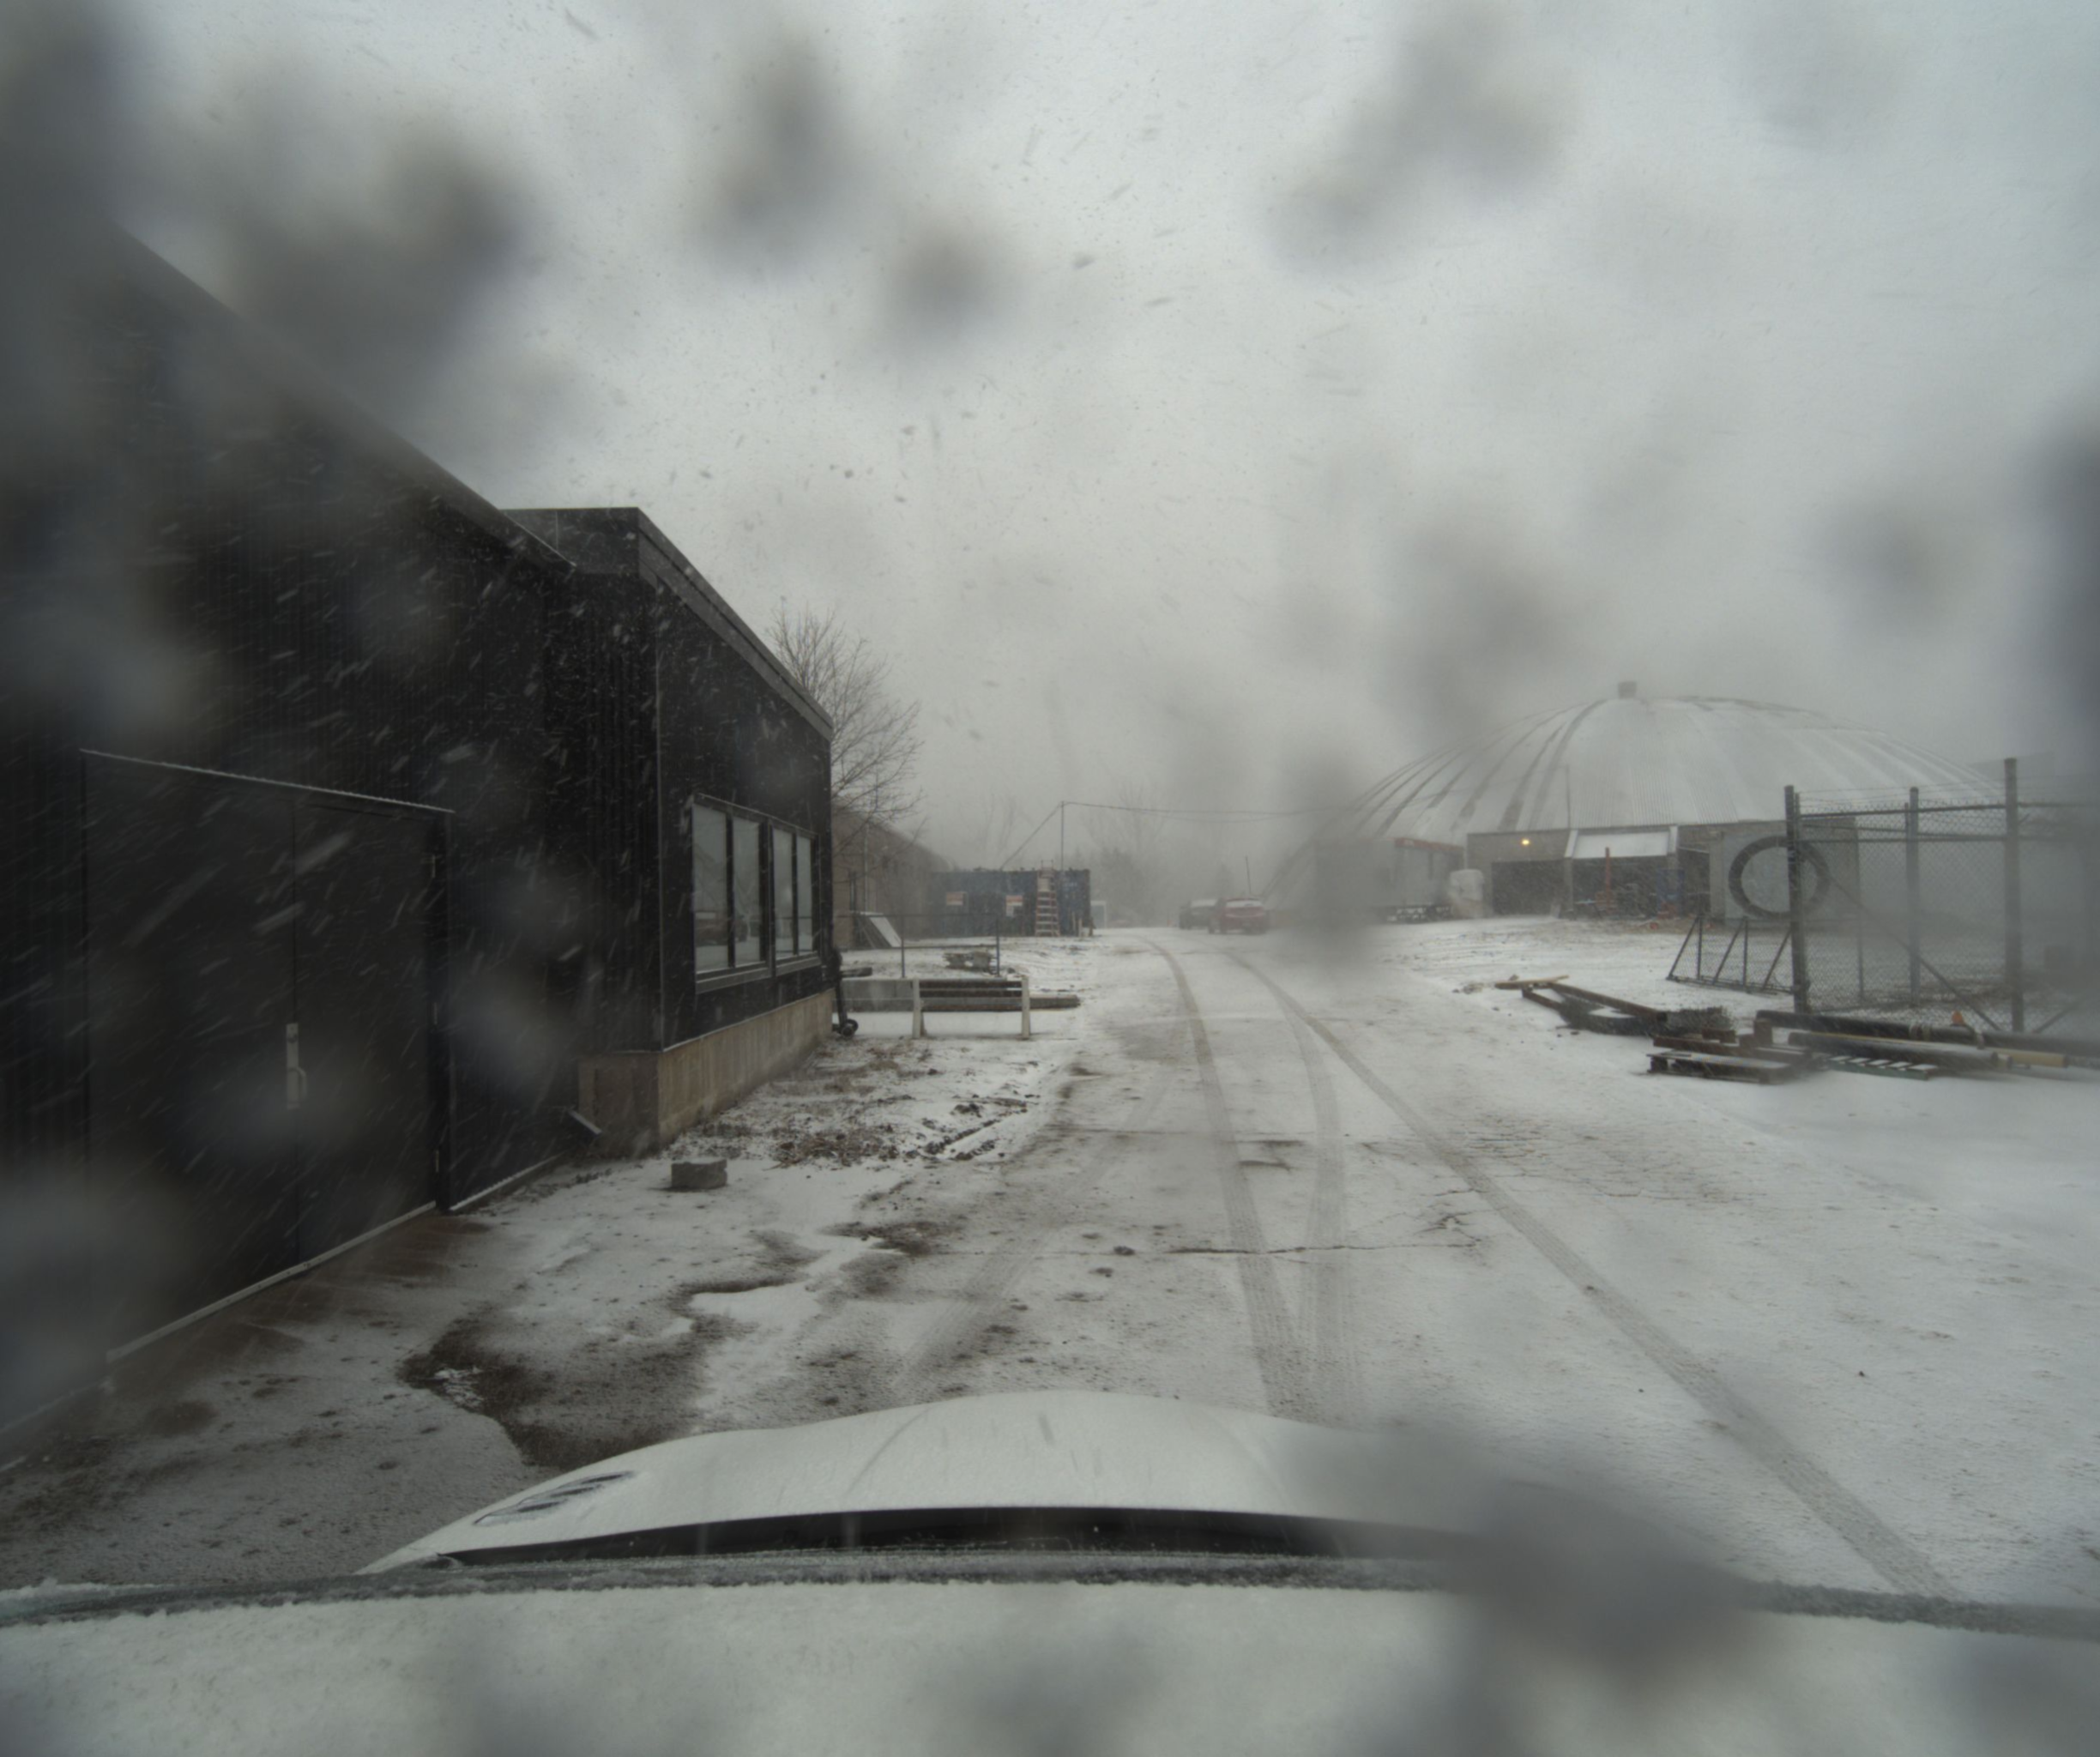
\includegraphics[width=\linewidth]{imgs/1611676774731026.png}
	\end{minipage}\hfill
	\begin{minipage}[b]{.45\linewidth}
		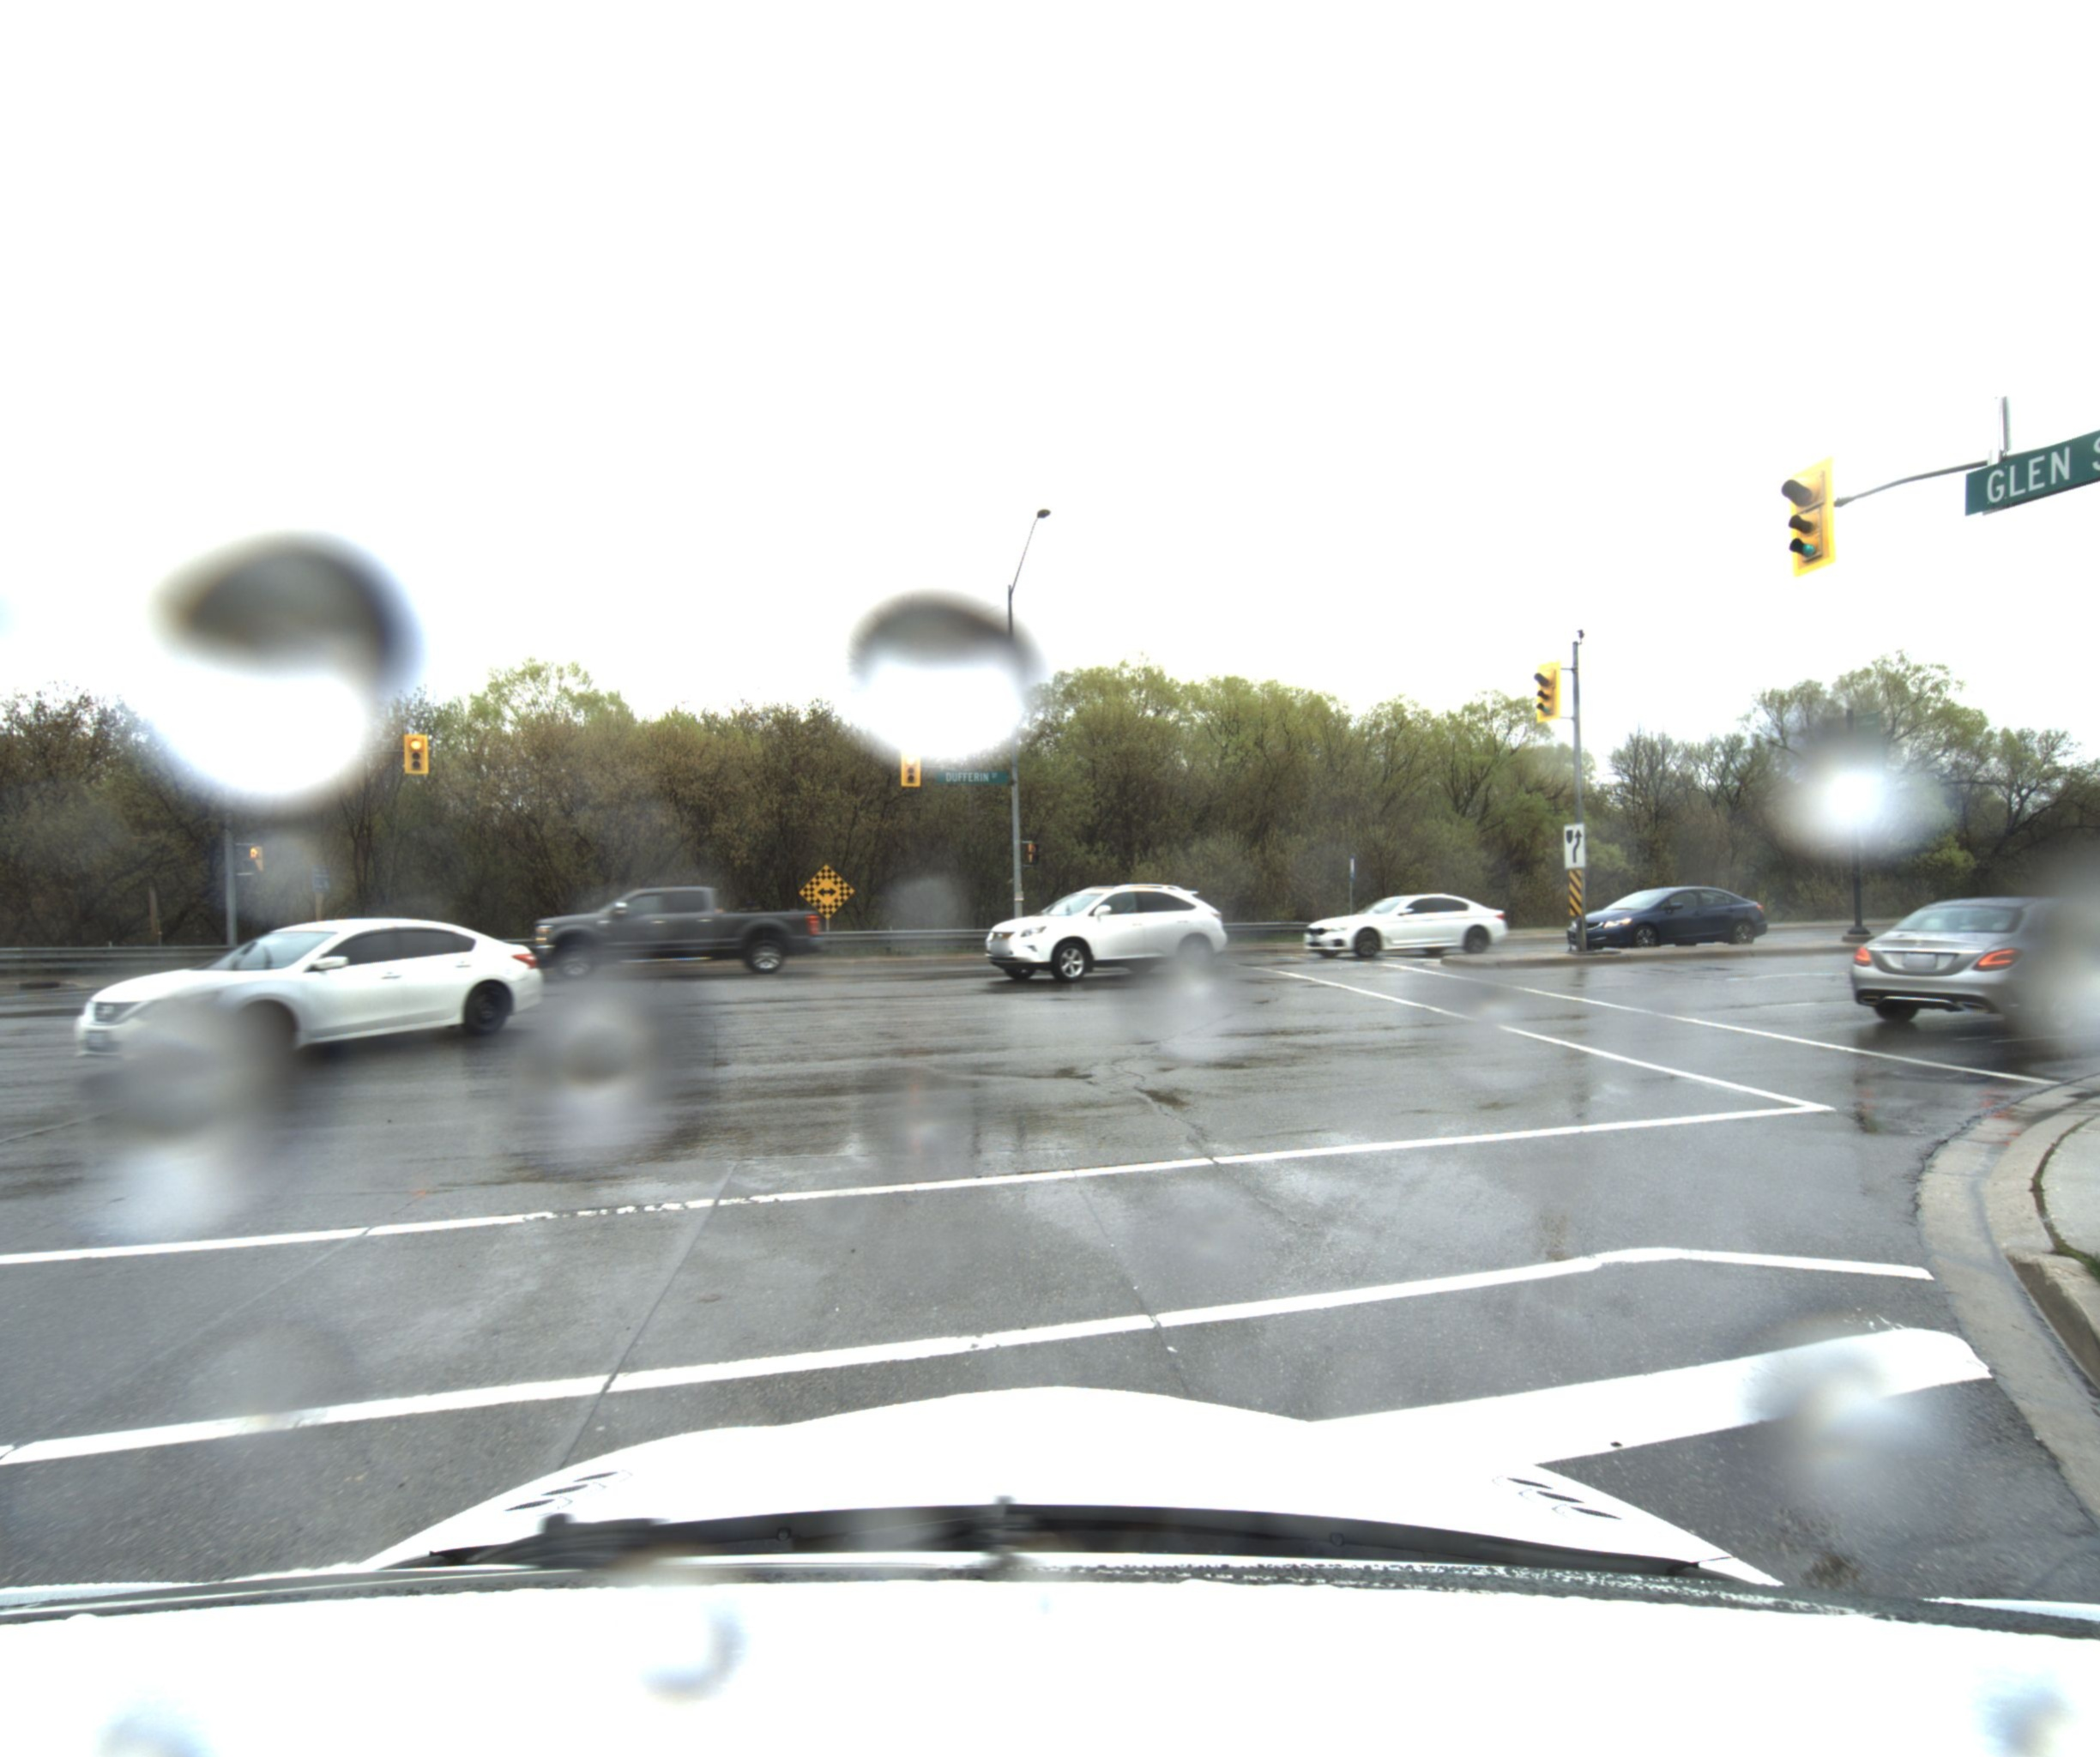
\includegraphics[width=\linewidth]{imgs/1619726918389964.jpg}
		
	\end{minipage}
	\caption{camera output in snow and rain weather conditions.}
	
	\label{img:rickety-camera}
\end{figure}

\section{Contributions}
Set up the Boreas dataset and modify the Pix2Pix and SPADE models to accept weather masks as input.
\section{Related Works} 

\chapter{Related Work}

\section{Related 1}

\section{Related 2}
 

% ---------- Anhang ----------

\begin{appendix}
	

\end{appendix}

% ---------- Verzeichnisse ----------

\listoffigures
%\listoftables
%\lstlistoflistings

% ----------------------------

% Erzeugt das Literaturverzeichnis
\printbibliography

% Erzeugt eine Seite mit der Erklaerung
\declaration{nutzung}

\end{document}
